% #############################################################################
% This is Chapter 7
% !TEX root = ../main.tex
% #############################################################################
% Change the Name of the Chapter i the following line
\fancychapter{Enhanced parameter-efficient transfer learning with Shared-Adapters}
\label{chap:7}
\cleardoublepage
%\section{Introduction}
In the preceding chapters, we demonstrated the effectiveness of Adapters, particularly residual Adapters, across various tasks associated with children's \ac{ASR}. These tasks encompassed \ac{PETL} for children's \ac{ASR} and mitigating domain mismatch for \ac{TTS} data augmentation. The success observed in these experiments has prompted a more in-depth analysis of potential alternatives to Adapters, additionally motivated by the literature, which offers alternative approaches that often yield superior performances and provide more parameter-efficient solutions for other tasks.
Indeed, the growing attention towards \ac{PETL} from the research community has led to the emergence of an array of novel architectures and methodologies. These alternatives extend beyond the conventional Adapters. These innovative approaches have been extensively explored in various domains such as \ac{NLP} and image processing but remain relatively unexplored in the domains of speech processing \cite{chen2023exploring} and even more for children's \ac{ASR}.

The objective of this chapter is to analyse these emerging \ac{PETL} methods specifically in the context of children's \ac{ASR}. Drawing from our prior findings, which underscored the significance of fine-tuning \ac{FFN} modules, we have curated a selection of \ac{PETL} approaches designed to be integrated with \ac{FFN} modules. Notably, we excluded \ac{PETL} approaches centred around the \ac{MHSA} modules, such as LORA \cite{hu2022lora}, as well as any prompt-related \ac{PETL} strategies like prompt tuning \cite{lester-etal-2021-power} or prefix tunning \cite{li-liang-2021-prefix}.

In this chapter, we introduce the Shared-Adapter, a novel approach for \ac{PETL} tailored for children's speech. Inspired by the redundancy inherent in the \ac{FFN} components of Transformer-based models \cite{pires2023one}, we hypothesise that the Adapters themselves would also exhibit redundancy. Therefore, we investigate the use of a single Adapter, shared across all the \ac{FFN}, independently of the layer. Through comprehensive experimentation, we assess the effectiveness of this approach in achieving a balance between model parameter reduction and preservation of recognition performance.

This chapter presents an in-depth presentation of the selected \ac{PETL}, alongside our novel Shared-Adapter, elucidating their underlying principles, architectural intricacies, and key characteristics compared to the traditional Adapter in the context of children's \ac{ASR}. The goal of this chapter is to answer the following research question: \textit{Which is the best approach for children parameter efficient \ac{ASR}? Can we propose a novel method that achieve state-of-the-art with fewer parameters?} The evaluation mainly encompasses two dimensions, the performances compared to the full-finetuning and the parameter-efficiency of the method. By systematically benchmarking these alternative \ac{PETL} methodologies against the conventional Adapter models, our objective is to not only understand the individual strengths and limitations of these approaches but also to evaluate their relative effectiveness in tackling the specific challenges presented by children's \ac{ASR}.

\section{Exploring PETL literature alternatives}
\label{section:petl_alt}
% general introduction of the two different types of new \ac{PETL} (mention here why LORA and prompt-based methods are not here) 
\subsection{Scaled Adapters}
% Explain the idea has been used in many examples
Scaled or Gated Adapters extend the conventional residual Adapters by introducing a scaling mechanism to the output of the Adapter modules. The concept of scaled-Adapters was initially introduced by He \textit{et al.} \cite{he2022towards} and is formally expressed as:
\begin{equation}
    adapter(x) = x + s \cdot (W_{up}(f(W_{down}g(x) + b_{down})) + b_{up})    
\end{equation}
% Tunable parameters
Here, $s \in \mathbb{R}$ is a tunable scalar hyperparameter. Notably, some research has proposed to learn directly this scalar value during training as a gate mechanism \cite{mao-etal-2022-unipelt}. The intuition behind this approach is to allow the network to gradually learn to assign weights to the target domain, achieving more fine-grained control of the Adapter activation or deactivation. The scaled learning process should facilitate the regulation of contributions from the Adapters from different layers, enabling the model to adapt and refine its responses based on the specific characteristics of the data encountered during training in a layer-wise fashion. Moreover, while the field of children's speech recognition has not yet explored gated or scaled Adapters, recent research has delved into more sophisticated gating processes for accented speech \ac{ASR} \cite{gong2022layer}, where the use of accent embeddings to regulate the gating mechanism.

% Experimental setup
Within the context of our experiments, we decided to use a trainable scalar associated with each Adapter module using a \ac{TPA} configuration in the Encoder only. These scaling parameters and all Adapter modules were optimised through 30 epochs of training using a learning rate of $8 \times 10^{-4}$.

\subsection{Convolution based Adapters}
% CNN make sense for speech
\acp{CNN} have been widely recognised for their effectiveness in exploiting local information, particularly for computer vision tasks \cite{9879745}. These networks learn shared kernels based on position within localised windows, giving them the ability to capture features such as edges and shapes. This characteristic has also been demonstrated in the field of speech-related tasks, as demonstrated by the success of the Conformer architecture \cite{gulati2020conformer}.

%Then CNN in Adapter is a normal step
As a result of this success, \acp{CNN} have been naturally incorporated into Adapter modules. This strategic fusion enables Adapters to leverage the spatial processing capabilities inherent in convolutional modules, thereby enhancing their capacity to capture and adapt to different patterns present in the data. The initial approach involved using \acp{CNN} as feature extractors within the Adapter module, in conjunction with a linear transformation \cite{yang23p_interspeech}. We denoted this approach as Conv-Adapter. First, we experimented with two versions of Conv-Adapter, where a 1-dimensional \ac{CNN} is used as a replacement of either the first or second linear of the traditional Adapters, respectively \textit{$\text{Conv-Adapter}_{Down}$} and \textit{$\text{Conv-Adapter}_{Up}$}. More formally, the \textit{$\text{Conv-Adapter}_{down}$} can expressed as followed:
\begin{equation}
    \text{Conv-adapter}_{Down}(x) = x + (W_{up}(\text{CNN}_{1D}(x))+ b_{up})
\end{equation}
While \textit{$\text{Conv-Adapter}_{up}$} is defined as:
\begin{equation}
    \text{Conv-adapter}_{up}(x) = x + \text{CNN}_{1D}(W_{down}(x)+ b_{down})
\end{equation}
We also investigated, the Conv-Adapter where the \ac{CNN} is integrated in-between the Up and Down projection of the traditional Adapter \cite{muthuchamyselvaraj23_interspeech}, denoted \textit{$\text{Conv-Adapter}_{Middle}$}, mathematically expressed as:
\begin{equation}
    \text{Conv-adapter}_{Middle}(x) = x + W_{up}(\text{CNN}_{1D}(W_{down}(x)+ b_{down})+ b_{up})
\end{equation}

\begin{figure}[h]
    \begin{center}
        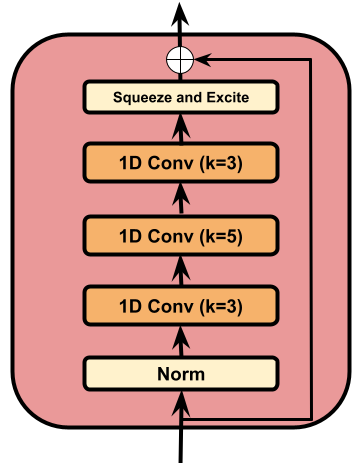
\includegraphics[scale=0.4]{imgs/ConvPass.png}
        \caption{The architecture of the ConvPass adapter. $k$ is the kernel size of the 1D convolution. All Convolutions are depth-wise convolutions.}
        \label{fig:convpass}
    \end{center}
\end{figure}

% Adapter fully CNN based
In addition to the Conv-Adapters, an alternative approach involves the use of a fully \ac{CNN}-based Adapter known as ConvPass, which has demonstrated effectiveness in computer vision tasks \cite{jie2022convolutional}. Diverging from conventional Adapters and the previously mentioned Conv-Adapter, ConvPass distinguishes itself by the removal of the up and down linear layers, replaced instead by three \ac{CNN} layers. In vision task \cite{jie2022convolutional}, these layers comprise a $1 \times 1$ convolution, followed by a $3 \times 3$ convolution, and another $1 \times 1$ convolution. With \ac{GELU} activation functions are interposed between these convolutional layers.

For speech-related tasks, a comparable approach was introduced by Li \textit{et al.} \cite{li2023evaluating}. The speech-specific ConvPass, illustrated in Figure \ref{fig:convpass}, incorporates a normalisation layer, followed by three lightweight 1-dimensional \ac{CNN} layers with kernel sizes of 3, 5, and 3, respectively. Additionally, a squeeze and excite module is integrated into the architecture. The squeeze and excite module \cite{hu2018squeeze}, facilitates feature recalibration. It consists of a global pooling operation, followed by a linear layer, a \ac{ReLU} activation, a second linear layer, and concludes with a Sigmoid activation.

During our experiments, all Conv-Adapters and ConvPass configurations were trained for 30 epochs with a learning rate of $8 \times 10^{-4}$ using a \ac{TPA} configuration in the Encoder only.


\subsection{BitFit}
Bias-Term Fine-Tuning, known as BitFit, is a \ac{PETL} method introduced for \ac{NLP} tasks \cite{ben-zaken-etal-2022-bitfit}. The main idea behind BitFit is to fine-tune only the bias terms and the task-specific classification layer while keeping the rest of the model frozen. This approach aims to achieve efficient fine-tuning with reduced computational requirements in a similar way as our partial fine-tuning experiments of Chapter \ref{chap:4}. The fine-tuning of bias terms can be seen as introducing a task-specific shift to the token representations.

%Advantages of Bitfit
The authors highlight three key properties of BitFit. Firstly, it matches a fully fine-tuned model on some \ac{NLP} tasks, showcasing its ability to maintain comparable results while significantly reducing the number of parameters to be trained. Secondly, BitFit is designed to adapt to tasks arriving sequentially, eliminating the need for simultaneous access to all datasets. This adaptability enhances the model's versatility in handling diverse tasks with varying data distributions over time. Thirdly, BitFit exhibits parameter efficiency by fine-tuning only a small subset of the model's parameters.

BitFit has been previously applied in various speech-related tasks \cite{cappellazzo2023parameter,hsieh23_interspeech}, including \ac{ASR} \cite{ng23c_interspeech2}. In these previous works, its performance varies depending on the specific task and datasets used in the experiments. However, there has been no dedicated evaluation of this approach's performance for children's \ac{ASR}, resulting in a knowledge gap that our experiment aims to answer.


%Experimental setup
In our experiment, the pre-trained model and children's \ac{ASR} task shared the same output dimensions and character encoding. In consequence, we excluded the fine-tuning of the task-specific classification layer concentrating solely on the tuning of the bias terms. The training process consisted of 30 epochs with a learning rate of $8 \times 10^{-4}$.

\subsection{Scale and Shift features}
% Define SSF
\ac{SSF} was introduced an \ac{PETL} alternative approach by Lian \textit{et al.} \cite{lian2022scaling} for image classification. The primary objective of \ac{SSF} is to establish a generalised method for efficient model fine-tuning without the introduction of task-specific inference parameters. Drawing inspiration from feature modulation techniques \cite{wu2018group,huang2017arbitrary}, the \ac{SSF} method modulates deep features extracted by a pre-trained model by scaling and shifting them to match the distribution of a target dataset. 
The intuition behind \ac{SSF} comes from the inherent disparities in data distributions between upstream and downstream datasets. Directly applying model weights trained on an upstream dataset to a downstream dataset frequently leads to performance degradation due to the disparities between the two datasets \cite{sun2016return}. The \ac{SSF} method addresses this challenge by introducing scale $\gamma$ and shift $\beta$ parameters, which could be considered as the variance and mean used to modulate the features extracted from the pre-trained model. This modulation ensures that the adapted features align with the characteristics of the upstream dataset. Formally, given an input $x$, the modulated output $y$ is calculated by:
\begin{align}
    y = \gamma \odot x + \beta
\end{align}

Notably, the scale and shift parameters in \ac{SSF} remain independent of any input and have a unified learnable parameter space for different tasks. Another notable advantage of \ac{SSF} is that the scale and shift weights can be seamlessly integrated into the original pre-trained weights of the linear layers during model re-parameterization in the inference phase. This integration avoids the need for additional parameters removing the extra-computation time of other \ac{PETL} such as Adapters. Importantly, it is noteworthy that the \ac{SSF} approach has not been previously applied to speech-related tasks.

% How to put it in a model
In practice, the \ac{SSF} modulations are introduced after each module of the Conformer architecture, namely the \acp{FFN}, \ac{MHSA} and Convolution modules. In the original paper, they also fine-tuned the head layers. However, as our upstream and downstream tasks, respectively adult and children \ac{ASR}, share the same output dimension and character encoding, we do not fine-tune this extra layer and we only use the \ac{SSF} method for each Conformer's modules. Our training compromises 30 epochs with a learning rate of $8\cdot10^{-4}$.

%Experimental setup
%In practice, the \ac{SSF} modulation is integrated after each operation of the neural network. For our experiments, each operation corresponds to the different modules within the Conformer architecture, specifically the \acp{FFN}, \ac{MHSA} and Convolution modules. It is noteworthy that, in the original paper, the authors also fine-tuned a head layer, as the output of the upstream and downstream image classification tasks are different. However, in our experiment, both the upstream and downstream tasks involve English \ac{ASR} with shared output dimensions and character encoding. Therefore, we did not include the head-layer fine-tuning and exclusively employed the \ac{SSF} method. Our training compromises 30 epochs with a learning rate of $8\cdot10^{-4}$.


\subsection{AdapterBias}
\begin{figure}[h]
    \begin{center}
        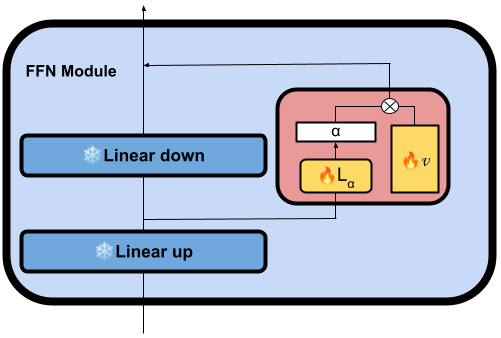
\includegraphics[scale=0.4]{imgs/AdapterBias.png}
        \caption{ AdapterBias, consisting of a linear layer $L_\alpha$ and a vector $\mathcal{V}$, is added after the second feed-forward layer only in each FFN module. The fire icon denotes trainable components, whereas the snow icon indicates frozen components.}
        \label{fig:AdapterBias}
    \end{center}
\end{figure}
% Link to Bitfit
Following the success of BitFit \cite{ben-zaken-etal-2022-bitfit}, which aims to introduce task-specific shifts to each output representation by selectively fine-tuning only the bias terms of a pre-trained model, recent research has suggested that certain tokens may hold more importance than others for specific tasks. While BitFit uniformly applies the same shift across all tokens regardless of their relevance to the task, AdapterBias were introduced to address this limitation \cite{fu-etal-2022-adapterbias}.

% What is AdapterBias
Compared to traditional residual Adapters, that are used in parallel or in series with the \ac{FFN} module, AdapterBias is plugged directly inside of the \ac{FFN} module, added after the second feed-forward layer only. In terms of design, AdapterBias comprises two essential modules: a vector $\mathcal{V}$ and a linear layer $L_\alpha$. The vector $\mathcal{V}$ represents a task-specific shift added to the output of each \ac{FFN} module. On the other hand, the linear layer $L_\alpha$ generates a token-dependent weight vector $\alpha = [\alpha_1, \alpha_2, ..., \alpha_m]^T$, where $\alpha_i$ is the weight associated with the shift of the $i^{th}$ token. By applying these token-specific weights to the task-specific representation shift $\mathcal{V}$, AdapterBias focuses on tokens which are more crucial to the task, allowing efficient and fine adaptation to various downstream tasks, as demonstrated in \ac{NLP} tasks \cite{fu-etal-2022-adapterbias}.

The output of AdapterBias is defined as the bias $B$ represented as the outer product of $\mathcal{V}$ and the learned weights vector $\alpha$ is summed to the outputs of the second feed-forward layer of the \ac{FFN} module. Mathematically, the output of AdapterBias $B$ is expressed as follows:

\begin{equation}
    B = \mathcal{V} \otimes \alpha^T    
\end{equation}

Here, $\otimes$ denotes the element-wise multiplication of the task-specific shift vector $\mathcal{V}$ and the token-dependent weight vector $\alpha$.


The effectiveness of AdapterBias for children's \ac{ASR} remains uncertain due to conflicting findings in existing studies. While some research suggests its efficacy in improving ASR performance \cite{chen2023exploring}, others have not observed significant benefits \cite{ng23c_interspeech2}. This discrepancy in findings suggests that the success of AdapterBias may depend heavily on factors such as the characteristics of the source and target domains. Therefore, there is a need for a dedicated evaluation of AdapterBias specifically for children's \ac{ASR} to understand its potential in addressing the unique challenges of children's speech. 


% Experimental setting
In our experimental setup, we conducted the training for AdapterBias by integrating them into the second linear layer of each of the two \ac{FFN} modules within the Conformer architecture. We trained AdapterBias for 30 epochs, employing a learning rate of $8 \times 10^{-4}$.

\subsection{Experimental setup}

In all experiments to assess the efficiency of \ac{PETL} alternatives, we employed the same pre-trained Conformer model outlined in Section \ref{section:TransformerConformerDetails}. As a training dataset, we used the My Science Tutor (MyST) Children's Speech Corpus. This dataset has been consistently used in prior experiments within the context of this thesis, and further details about the MyST corpora are provided in Section \ref{section:children_corpora}.

\subsection{Results of the different PETL methods}

\begin{figure}[h]
    \begin{center}
        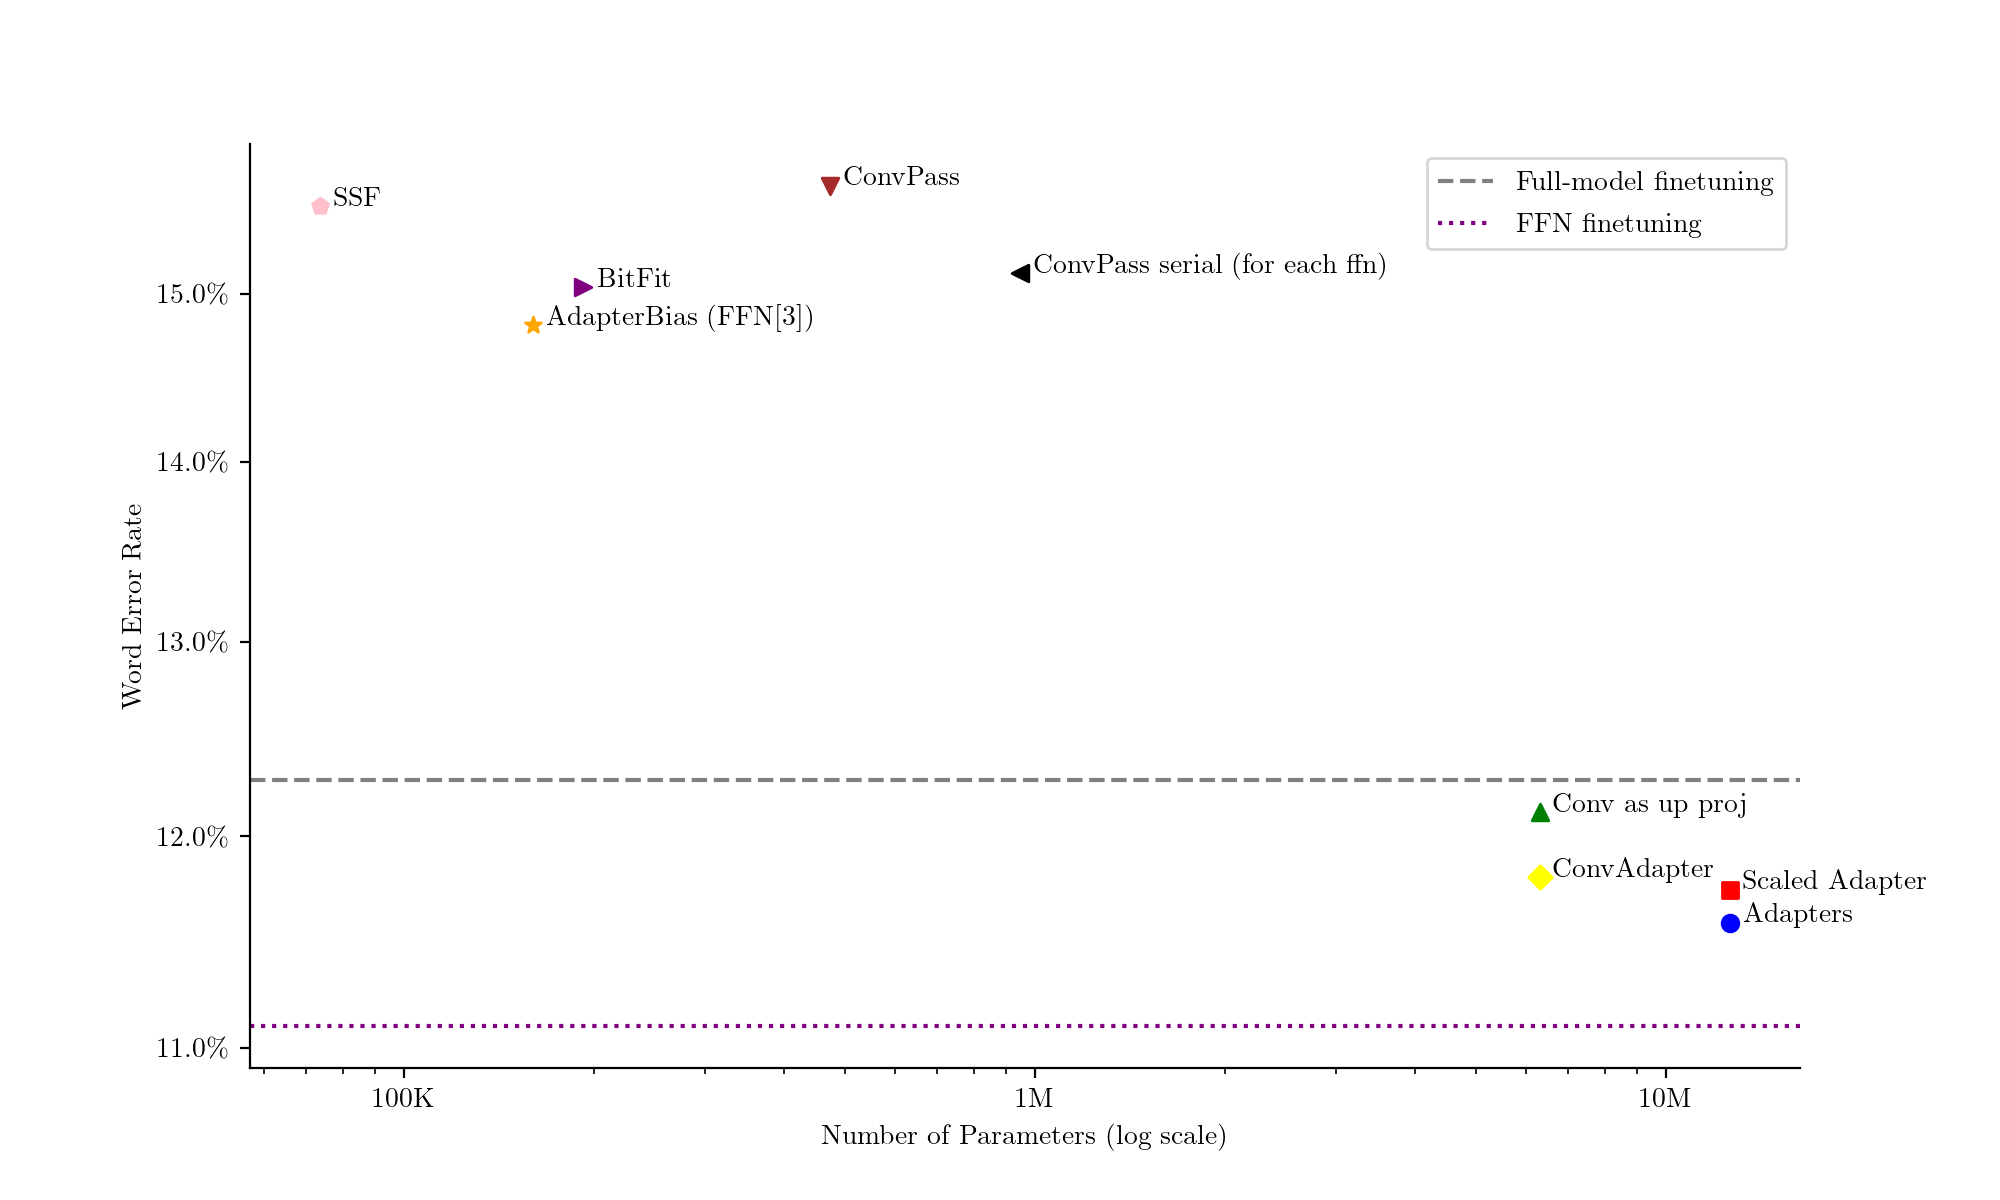
\includegraphics[width=\textwidth]{imgs/Adapter_compare_withoutWide.png}
        \caption{Different parameter efficient procedure for children ASR in Conformer model}
        \label{fig:adapter_compared_withoutWide}
    \end{center}
\end{figure}
\begin{table}[h]
    \centering
    \begin{tabular}{lccc}
        \toprule
        \textbf{PETL Method} & \textbf{WER $\downarrow$} & \textbf{Trained Parameters} \\
        \midrule
        Full fine-tuning & 12.28 & 109.1M \\ \hline
        Adapter & \textbf{11.58} & 12.6M \\
        Scaled Adapter & 11.74 & 12.6M \\
        ConvAdapter(Down) & 12.03 & 6.4M \\
        ConvAdapter (Middle) & 11.62 & 12.7M \\
        ConvAdapter (Up) & 11.78 & 6.4M \\
        ConvPass & 15.13 & 946.2K \\
        BitFit & 15.04 & 192K \\
        SSF & 15.55 & 73.7K \\
        AdapterBias & 14.81 & 159.8K \\
        \bottomrule
    \end{tabular}
    \caption{WER performances and number of parameters of the different PETL alternatives on children ASR. WER expressed in terms of percentage.}
    \label{tab:PETL_alternatives}
\end{table}
% Adapter and Scaled Adapter
The results of various \ac{PETL} methods are summarised in Table \ref{tab:PETL_alternatives}. Notably, the traditional residual Adapter approach using the \ac{TPA} configuration emerges as the most effective, achieving an 11.58\% \ac{WER} with 12.6 million parameters. The Scaled Adapter method exhibits a slightly reduced \ac{WER} performance at 11.74\% while maintaining the same parameter count of 12.6 million.

%ConvAdapter and ConvPass
Turning attention to convolution-based Adapters, the replacement of either linear layer ($W_{down}$ and $W_{up}$) results in decreased performance, yielding WERs of 12.02\% and 11.78\%, respectively, using both 6.4 million parameters. Interestingly, introducing a convolutional layer between these two linear layers proves to be the best-performing convolutional system, approaching the scores of the regular Adapter with 11.62\% \ac{WER} and using a slightly increased amount of parameters of 12.7 million. It is noteworthy that all these Conv-Adapter setups and the Scaled Adapters approach continue to outperform the fine-tuning of the entire model and are therefore valuable approaches for children's \ac{ASR} \ac{PETL}.
On the other hand, the ConvPass method, where all linear layers of the Adapter were replaced by convolution layers, did not surpass the full fine-tuning, yielding a \ac{WER} of 15.13\% with 946.2 thousand parameters.

% Bitfit, SSF and AdapterBias
Moving to bias shift methods, such as BitFit, \ac{SSF}, and AdapterBias, these approaches underperformed compared to the entire model fine-tuning, with respective \acp{WER} of 15.04\%, 15.55\%, and 14.81\%. However, it is important to note that these methods use significantly fewer parameters, with 192, 73.7, and 159.8 thousand parameters, respectively.

% Summary
In summary, the traditional residual Adapter remains the most effective \ac{PETL} approach for children's \ac{ASR}. This finding aligns with recent research, as highlighted different studies \cite{li2023evaluating,cappellazzo2023parameter}, which also affirm the superior performance of Adapters in \ac{PETL} for \ac{ASR} tasks. Moreover, our findings highlight a noticeable trade-off between the number of parameters and the \ac{WER}. Specifically, approaches employing fewer than a million parameters did not exhibit comparable performances to entire model fine-tuning or other \ac{PETL} methods with more parameters, as illustrated explicitly in Figure \ref{fig:adapter_compared_withoutWide}. This trade-off emphasises the need for more research on the development of \ac{PETL} methods that can effectively use fewer parameters while simultaneously maintaining or enhancing performance in the domain of children's \ac{ASR}.

\section{Leveraging Transformer-based model redundancy for Shared-Adapter}
\subsection{Shared-Adapter}
% Goal PETL- Good score, small |param|
The primary objective of \ac{PETL} is to either maintain or surpass the performance achieved through full fine-tuning of a pre-trained model while minimising the number of parameters employed during training. In the previous section, the efficiency of residual Adapters has been underscored. Remarkably, using only 10\% of the total number of parameters compared to the fine-tuning of the entire model, these residual Adapters exhibit superior performances in the context of children's \ac{ASR}. In addition, our findings, particularly from Chapter \ref{chap:4},  highlighted the drawback of overparameterisation present in Transformer-based models.

% FFN redundancy
Additionally, researchers found that the \ac{FFN} modules, despite constituting a significant proportion of the model's parameters, were identified as highly redundant \cite{pires2023one}. This affirmation was corroborated by the work of Geva and al. , which establishes a connection between the \ac{FFN} and attention mechanisms \cite{geva2020transformer}. The latter proposes that the \ac{FFN} can be conceptualised as learnable key-value memories, with the weights of the first linear layer representing keys and those of the second layer corresponding to values. These keys are proficient at capturing salient patterns at each layer. Interestingly, they observed that the classes of patterns tend to overlap between neighbouring layers, indicating redundancy in the representations. This observation underscores the potential for optimising \ac{PETL} methods by addressing and mitigating redundancy within \ac{FFN} modules.

% Shared FFN work
Building upon these observations, Pires and al. modified the Transformer architecture by sharing and dropping the \ac{FFN} across different layers \cite{pires2023one}. Their investigation confirms the substantial degree of redundancy between the \acp{FFN} of the Encoder and Decoder components. Consequently, they successfully eliminate the Decoder \ac{FFN} while sharing a single \ac{FFN} across the Encoder, achieving a noteworthy reduction in model parameters without significant compromise to accuracy.

Formally, with $N_{enc}$ denoting the number of Encoder layers, the sharing of the \ac{FFN} modules in the Encoder can be expressed as follows:

\begin{equation}
    \text{FFN}_{i}^{enc}(.) \stackrel{\text{tied}}{=} \text{FFN}^{enc}_{all}(.) , \forall i: 1 \leq i \leq N_{enc}
\end{equation}

%Shared Adapter motivation
In light of the success observed with the shared \ac{FFN} in the Encoder, we hypothesise that the presence of redundancy within the \ac{FFN} might lead to a similar redundancy issue when employing one Adapter per \ac{FFN} module. In other words, employing separate Adapters plugged into redundant \ac{FFN} modules for different layers might also exhibit redundancy within the different Adapters. To address this concern, we introduced the \textit{Shared Adapter} approach, wherein a single residual Adapter is used across all layers as shown in figure \ref{fig:adapter_compared}. This approach aims to use the redundancy present in \ac{FFN} layers modules to reduce the total amount of parameters used in Adapter-transfer. The formal expression of the Shared Adapter is presented as follows:

\begin{equation}
    \text{Adapter}_{i}(.) \stackrel{\text{tied}}{=} \text{Shared-Adapter}_{all}(.) , \forall i: 1 \leq i \leq N_{enc}
\end{equation}

% Compared to traditional adapter + Hidden dimension + Number of hours
In order to evaluate our proposed approach, our initial focus is on comparing the Shared-Adapter configuration with full fine-tuning and the Traditional Adapter. Subsequently, we vary the hidden dimension of the Shared-Adapter to assess how the number of parameters and the hidden dimension influence the performance. This comprehensive analysis aims to provide insights into the effectiveness of Shared-Adapters across various scenarios and configurations. Finally, we assess the robustness of both Traditional and Shared-Adapters by examining their performance under different amounts of training data, simulating low and extremely low resource scenarios.

\subsection{Experimental setup}
\begin{figure}[h]
    \centering
    \subfigure[Shared-Adapter setup in a Conformer model]{\label{fig:Shared_adapter}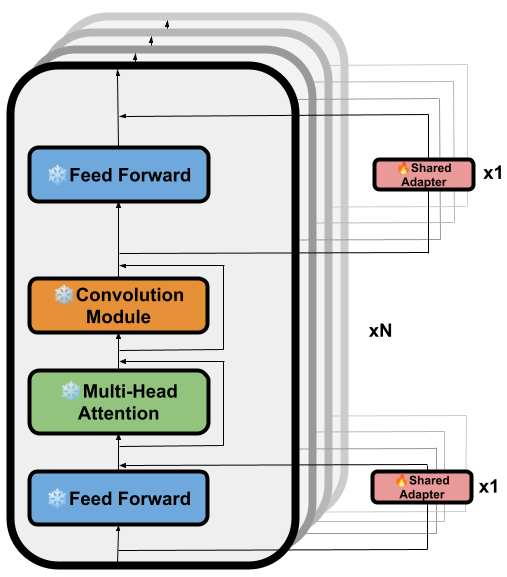
\includegraphics[width=0.45\textwidth]{imgs/Shared_Adapters.png}}
    \subfigure[Light Shared-Adapter setup in a Conformer model]{\label{fig:extrem_adapter}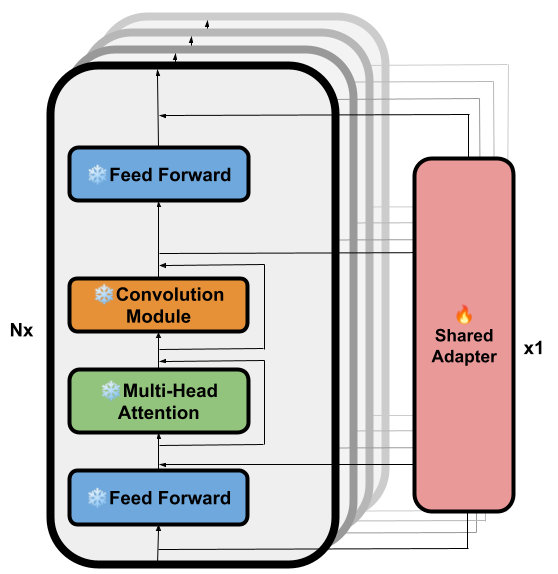
\includegraphics[width=0.48\textwidth]{imgs/Extreme_shared_adapter.png}}
    \caption{Overview of the Shared Adapters configurations. The fire icon denotes trainable components, whereas the snow icon indicates frozen components.}
\end{figure}


In our analysis, we focus on evaluating the performance of the Shared-Adapter using the same setting as the \ac{TPA} configuration for traditional Adapters. Especially because the \ac{TPA} configuration was found to be the most effective in Conformer models. Specifically, we assess the Shared-Adapter within a Conformer \ac{ASR} model, where two Shared-Adapters are directly integrated into the two \ac{FFN} modules for all layers as shown in Figure \ref{fig:Shared_adapter}.  The hidden dimension of the Shared-Adapters is set to 512. In terms of \ac{ASR}, we used the same Conformer model as the rest of the thesis, which comprises 12 Conformer layers followed by 6 Transformer layers. As we solely want to asses the performances of Shared-Adapters to model acoustics variabilities of children's speech, we exclusively evaluate the Shared-Adapter in the Encoder only.

To quantify the reduction of the number of parameters used in the Shared-Adapter compared to the traditional Adapter, the following formula is used:
\begin{equation}
    \text{Number of Parameters in Shared-Adapter} = \frac{\text{Number of Parameters of all traditional Adapters}}{\text{Number of Layers}}
\end{equation}

In addition, we propose an extension of the novel Shared-Adapters concept within the \ac{TPA} configuration. This novel approach, called \textit{Light Shared-Adapter} involves using a single Adapter for all \ac{FFN} modules instead of two, shared by the first and second \ac{FFN} modules. This configuration has the potential to further reduce the number of parameters by half compared to the use of two Shared-Adapters in the \ac{TPA} setup. This Light Shared-Adapter configuration is represented in Figure \ref{fig:extrem_adapter}. The \textit{Light Shared-Adapter} exploration aims to test the limits of the parameter efficiency and accuracy balance of our approach within the context of children's \ac{ASR}. 

In terms of the number of parameters, while the traditional Adapter uses approximately 12.6 million parameters, the number of parameters employed by the Shared-Adapter transfer is approximately 1.1 million and the Light Shared-Adapter uses only 527.9 thousand parameters. This represents a substantial reduction, as the Shared-Adapter and Light Shared-Adapter configurations use only 8\% and 3\%, respectively, of the number of parameters of the traditional Adapters setup. Moreover, considering that the traditional Adapter already represents approximately 10\% of the total parameters used in the entire model fine-tuning, the Shared-Adapter and Light Shared-Adapter configurations use only 1\% and 0.5\%, respectively, of the trainable parameters when compared to the entire model fine-tuning. This reduction in the number of parameters highlights the high parameter efficiency gains achieved by these novel configurations. For training all our different systems, we use 30 epochs with a learning rate set to $8 \times 10^{-4}$, in addition to a fixed hidden dimension of 512.

\subsection{Results}
\subsubsection{Shared-Adapter compared to other PETL methodologies}
\begin{figure}[h]
    \begin{center}
        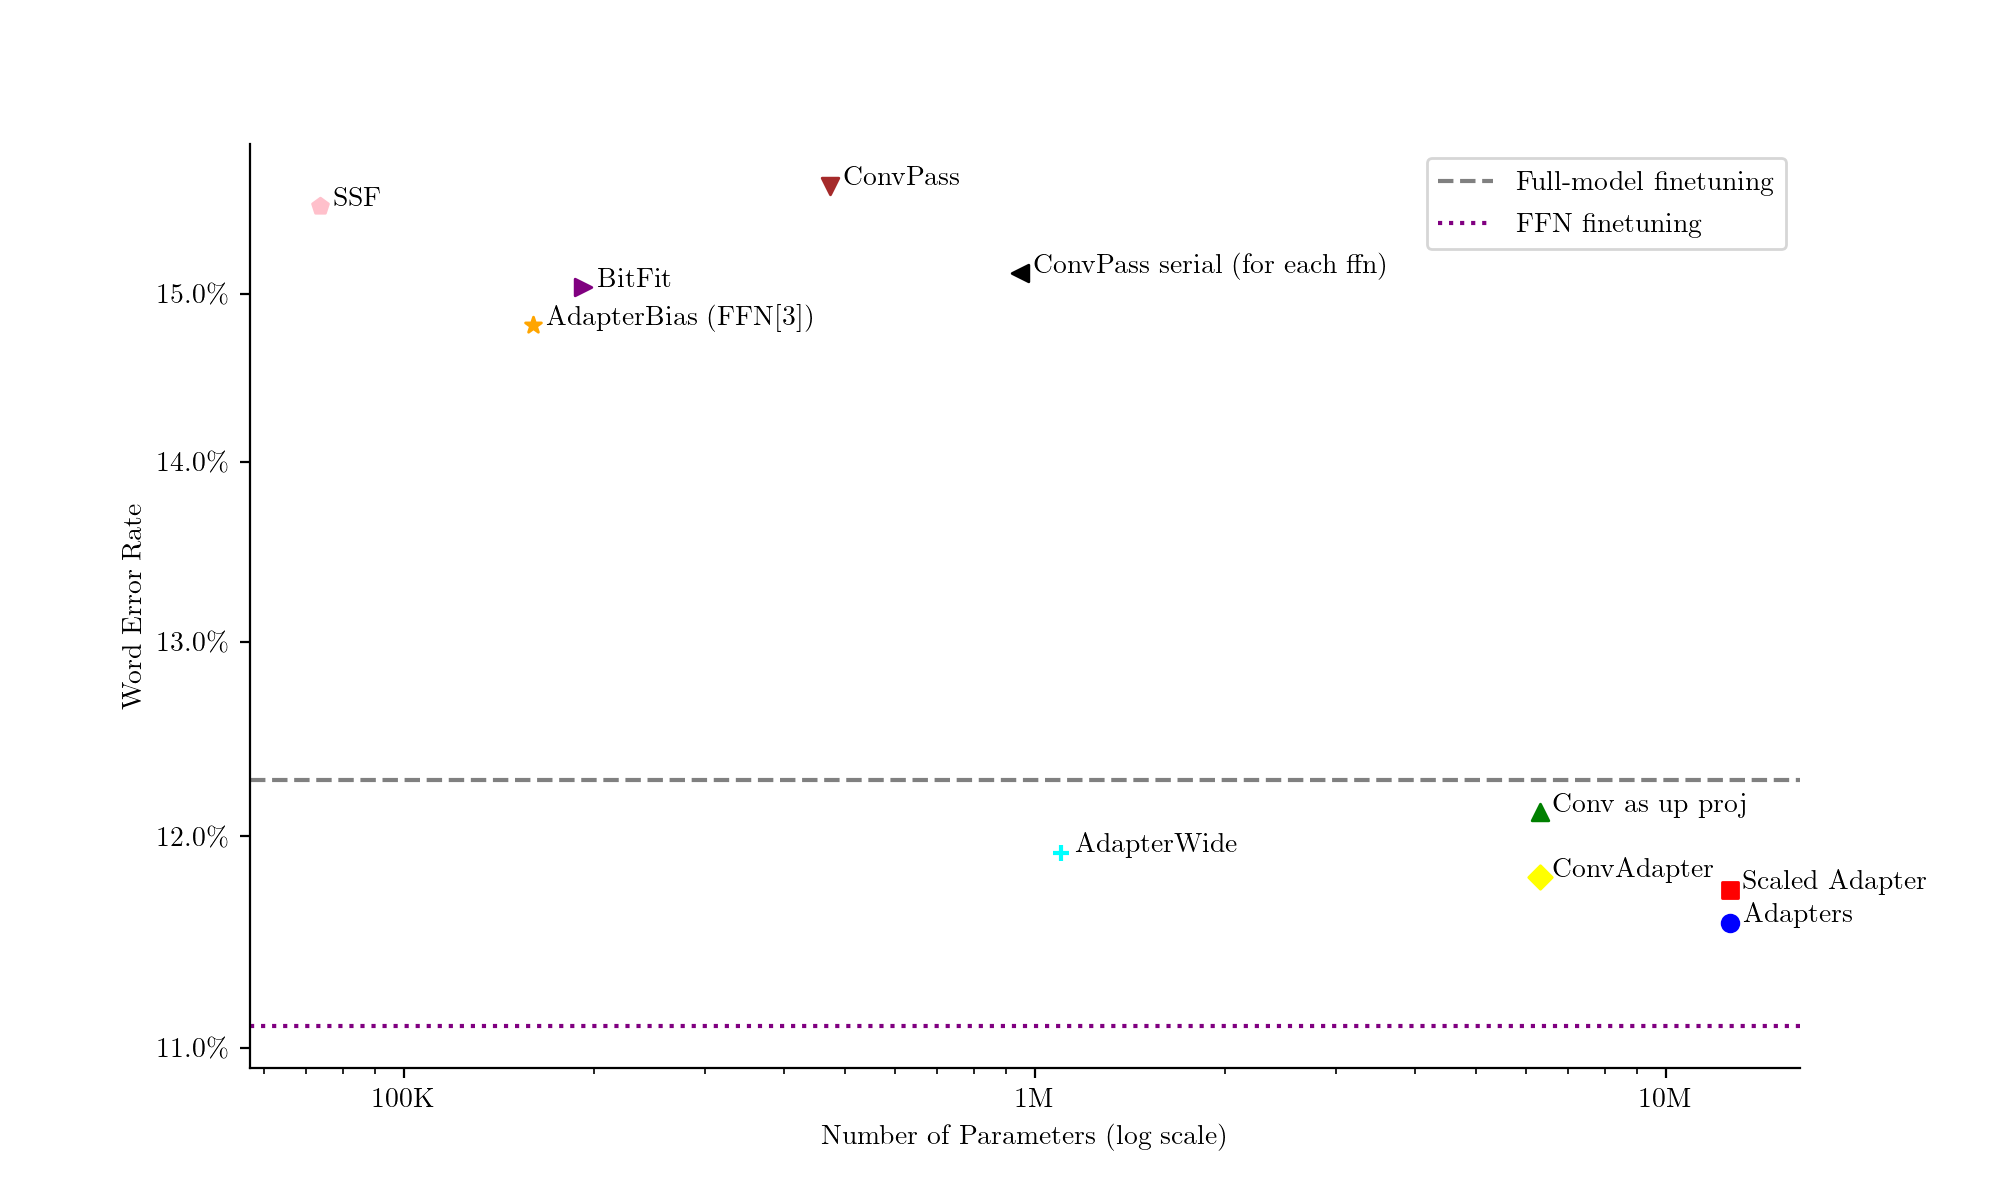
\includegraphics[width=\textwidth]{imgs/Adapters_compare.png}
        \caption{Different parameter efficient procedures for children ASR in Conformer model compared to the Shared-Adapters and Light Shared-Adapters}
        \label{fig:adapter_compared}
    \end{center}
\end{figure}

\begin{table}[h]
    \centering
    \begin{tabular}{l c c c}
        \hline
        \textbf{Configuration} & \textbf{WER $\downarrow$} & \textbf{Trained Params} \\
        \hline
        Full Fine-tuning & 12.28 & 109.1M \\ \hline
        Traditional Adapter & \textbf{11.58} & 12.6M \\
        Shared-Adapter & 11.92 & 1.1M \\
        Light Shared-Adapter & 12.31 & 526.3K \\ \hline
    \end{tabular}
    \caption{WER and Parameters for the Shared-Adapter and Light Shared-Adapter compared to traditional Adapter and full model fine-tunning. WER expressed in terms of percentage.}
    \label{tab:shared_adapter_results1}
\end{table}

In our comprehensive analysis, we systematically evaluated the efficacy of our proposed Shared-Adapter configuration against established \ac{PETL} methods mentioned in Section \ref{section:petl_alt}. The comparison, illustrated in Figure \ref{fig:adapter_compared} and presented in Table \ref{tab:shared_adapter_results1}, highlights the remarkable performance of the Shared-Adapter, particularly in achieving a notable balance between parameter efficiency and accuracy. Notably, the Shared-Adapter outperforms full-model fine-tuning while using only 1\% of the entire model's number of parameters, a significant reduction compared to the 10\% used by the Adapters. Although the Light Shared-Adapter exhibits a marginal degradation, surpassing the \ac{WER} of the entire model fine-tuning, it still outperforms alternative methods such as ConvPass, BitFit, AdapterBias, and \ac{SSF} by a considerable margin. These findings emphasise the efficiency of the Shared-Adapter as a novel parameter-efficient strategy, demonstrating a superior balance compared to existing methodologies. 

\subsubsection{Evaluating the hidden dimension and parameter influence on Shared-Adapter}
\begin{table}[h]
    \centering
    \begin{tabular}{l c c c}
        \hline
        \textbf{Configuration} & \textbf{WER $\downarrow$} & \textbf{Trained Params} \\
        \hline
        Traditional Adapter 512 & \textbf{11.58} & 12.6M \\ \hline
        Shared-Adapter 128 & 12.74 & 265.5K \\
        Shared-Adapter 256 & 12.34 & 527.9K \\
        Shared-Adapter 512 & 11.92 & 1.1M \\
        Shared-Adapter 1024 & 11.90 & 2.1M \\
        Shared-Adapter 2048 & 11.86 & 4.2M \\
        Shared-Adapter 4096 & \textbf{11.83} & 8.4M \\
        Shared-Adapter 6144 & 11.88 & 12.6M \\ \hline
    \end{tabular}
    \caption{WER and Parameters for different Shared-Adapter hidden dimension. WER expressed in terms of percentage.}
    \label{tab:shared_adapter_results}
\end{table}


The results in Table \ref{tab:shared_adapter_results} present the performance of different configurations of the Shared-Adapter model with varying hidden dimensions compared to Traditional Adpater and full model fine-tuning. As mentioned in the previous section, Shared-Adapter and Light Shared-Adapter achieved remarkable performances compared to Traditional Adapters and the full model fine-tuning while using fewer parameters. Additionally, as we decrease the hidden dimension to 128, the WER increases slightly to 12.74\% \ac{WER}, with a reduction in the number of trained parameters to 265.5K. Interestingly, as the hidden dimension increases from 128 to 4096, the \ac{WER} consistently decreases. In particular, the Shared-Adapter with a hidden dimension of 4096 exhibits the best performance, achieving a \ac{WER} of 11.83\%, with a larger parameter count of 8.4M. 
However, as we push the hidden dimension further to 6144, giving an equivalent number of parameters as the Traditional Adapters, the performance starts to degrade. We also observed, a drop in score compared to the Traditional Adapters setup for the same number of parameters. This decline and drop in performance when using a large hidden dimension suggests a tipping point where the model's capacity to effectively learn relevant information becomes more challenging.

%The results suggest that increasing the hidden dimension in the Shared-Adapter model generally improves its performance in terms of \ac{WER}, reaching a notable best performance at a hidden dimension of 4096. However, this improvement comes at the cost of a substantial increase in the number of trained parameters. Therefore, our results underscore the nuanced relationship between the hidden dimension, model performance, and the associated number of parameters where the hidden dimension needs to be carefully selected. 

\subsubsection{Low resource and extremely low resource scenarios robustness}
\label{sec:hours_PETL}
\begin{table}[h]
    \centering
    \begin{tabular}{l c c c}
        \hline
        Number of hours & Fine-tune (109.1M) & TPA Adapter (12.6M) & Shared-Adapter (1.1M) \\
        \hline
        1h & 16.24 & 16.51 & 17.20 \\
        10h & 14.00 & 14.05 & 14.28 \\
        20h & 13.43 & 13.30 & 13.52 \\
        50h & 12.94 & 12.40 & 12.57 \\
        All (\~113h) & 12.28 & 11.58 & 11.92 \\
        \hline
    \end{tabular}
    \caption{WER for different training durations for the full model fine-tune, TPA Adapter, and Shared-Adapter. WER expressed in terms of percentage.}
    \label{tab:training_duration_results}
\end{table}

To assess the effectiveness of Adapter-transfer and the Shared-Adapter in settings with limited and extremely limited resources, we conducted training with varying amounts of training data. The results are outlined in Table \ref{tab:training_duration_results}. We considered three methodologies: Full model fine-tuning, Traditional Adapters using the \ac{TPA} configuration, and Shared-Adapter, which also employed a \ac{TPA} configuration with one Shared-Adapter per \ac{FFN} module. The experiment covered scenarios with 50 and 20 hours, representing low-resource settings, and extremely low-resource scenarios with only 10 and 1 hour for training.

For full model fine-tuning, the \ac{WER} ranges from 16.24\% with 1 hour of training to 12.28\% with the entire training set (approximately 113 hours). In parallel, Traditional Adapters show a \ac{WER} reduction from 16.51\% to 11.58\% across the same durations. Notably, in extremely low-resource scenarios, Adapters and full transfer learning yield comparable results. Conversely, Adapters start to outperform the full model fine-tuning when the training duration exceeds 20 hours, reaffirming the efficiency of Adapter transfer for children's \ac{ASR}. The difficulty in training Adapter-based configurations, particularly in scenarios with less than 20 hours of data, may arise due to the need to train Adapter modules from scratch with randomly initialised weights. 

The Shared-Adapter model exhibits competitive performances in all scenarios, with a \ac{WER} decrease from 17.20\% to a notable 11.92\% as training duration extends. This establishes Shared-Adapter as a robust \ac{PETL} approach even in low-resource and extremely low-resource scenarios of children's speech.

\section{Summary and discussion}
% Summary
In this chapter, we addressed the following research question: \textit{Which is the best approach for children parameter efficient \ac{ASR}? Can we propose a novel method that achieve state-of-the-art with fewer parameters?}. The comprehensive evaluation of various parameter-efficient transfer learning alternatives from the existing literature revealed that these alternatives did not surpass the performance achieved by traditional Adapter modules. Furthermore, our results on children's \ac{ASR} highlighted the presence of an important tradeoff between accuracy and parameter efficiency.

Crucially, the optimal balance was observed when \ac{PETL} methods used around 10\% of the total parameters of the entire pre-trained model. This parameter-efficient configuration consistently resulted in \ac{WER} scores below those obtained through the full-model fine-tuning. However, reducing the proportion of parameters trained to less than 10\% of the full model led to a notable deterioration in \ac{WER} scores, underlining the tradeoff between parameter efficiency gains and preservation of accuracy in children's \ac{ASR} systems.


Additionally, we introduced a novel \ac{PETL} approach, the Shared-Adapter. Leveraging the inherent redundancy of \ac{FFN} modules in between the different Transformer layers. Our experimental evaluation demonstrated that Shared-Adapters represent a breakthrough in parameter efficiency while maintaining high accuracy in children's \ac{ASR}. Notably, while conventional \ac{PETL} methods typically required around 10\% of the total amount of the entire model parameters, Shared-Adapters excelled by achieving comparable accuracy with only 1\% of the parameters. Pushing the boundaries even further, we explored the extreme scenario of using the Light Shared-Adapters configuration with a mere 0.5\% of the model's total parameters, yet still achieving performance levels similar to full-model fine-tuning. Our approach eliminates the need for the aforementioned tradeoff, offering a pathway to obtain superior parameter efficiency without compromising accuracy.

% Discussion
The remarkable success of the Shared-Adapter approach underscores the significant redundancy of the \ac{FFN} modules across different layers. This new understanding is pivotal for advancing the development of more efficient, computationally compact \ac{ASR} models. Future research directions could explore the creation of a novel Transformer architecture designed to address the observed redundancy, providing an architecture that is inherently easier to fine-tune for children's \ac{ASR} or speaker-specific tasks. Additionally, investigating a new approach that incorporates both Shared and non-shared Adapters at the same time represents another avenue for potential advancements in the field. These avenues hold promise for enhancing the efficiency and robustness of \ac{ASR} models, particularly in contexts with limited data.